\chapter{Stationary states classification within symbolic dynamics framework}

\section{Objections}

In this chapter we describe an approach that is used further in order to classify all stationary state of one-dimensional GPE that are described by the stationary states equation:
\begin{equation}
	u_{xx} + Q(x) u + P(x) u^3 = 0.
	\label{eq:stationary}
\end{equation}
Here and after we assume $Q(x)$, $P(x)$ to be periodic functions of the same period $L$: $Q(x + L) = Q(x)$, $P(x + L) = P(x)$ which is quite typical for different physical applications.
We also assume functions $Q(x)$, $P(x)$ to be at least piece-wise continuously differentiable.
That allows us to split the whole real axis $\mathbb{R}$ into separate intervals where the corresponding Cauchy problem correctly defined and a solution for any initial conditions exists and is unique within each such interval.

Our classification approach is based on the technique proposed in the work \cite{AlfimovAvramenko}.
In \cite{AlfimovAvramenko} authors show that presence of a large number of singular solutions families allows to classify all remaining bounded solutions within a symbolic dynamics framework.
That leads us to another important requirement, function $P(x)$ must {\it changes its sign along the period} $L$.
As we saw in the previous chapter such fact guarantees the existence of singular solution families that in its turn becomes a foundation of the technique and makes the announced approach even possible.

Goal of this chapter is to provide a stationary states classification framework and point out the boundaries of its application.
Core idea is the following.
We define a Poincar\'e map $\mathcal{P}$ for the stationary states equation \eqref{eq:stationary}.
Since function $P(x)$ alternates its sing, Poincar\'e map $\mathcal{P}$ and an inverse map $\mathcal{P}^{-1}$ cannot be defined on the whole phase plane, instead they are defined on some phase plane subset.
Studying the domains of maps $\mathcal{P}$, $\mathcal{P}^{-1}$ is a crucial aspect of the proposed approach.
We determine conditions which allow to conclude that Poincar\'e map acts on the defined set as a kind of the {\it horseshoe map} \cite[Chapter 5]{GuekenheimerHolmes}.
Domains of the higher order maps $\mathcal{P}^2,~\mathcal{P}^3, \dots$ and domains of the inverse maps $\mathcal{P}^{-2},~\mathcal{P}^{-3}, \dots$ can be obtained by the refinement of the initial area.
Finally if some conditions are met and we can conclude that there exists one-to-one correspondence between all bounded solution of the equation \eqref{eq:stationary} and a points set on the phase plane which is a result of the above mentioned refinement.
That is what we call singular solution elimination method.

The presence of the horseshoe map structure allows us for each bounded solution uniquely specify a bi-infinite symbolic sequence over some alphabet (finite or even infinite) and such correspondence is also bijective.
We refer to the result bi-infinite sequence as {\it solution code} and the overall process as {\it solutions coding}.
Such coding, if possible, provides a complete picture of the bounded solutions family for the equation \eqref{eq:stationary} that can be highly demanded in different physical applications which involves Gross-Pitaevskii equation with both periodic potential and periodic pseudopotential.

\section{Geometry of the Poincar\'e map}

First of all let's introduce several definition which define basic structures and their relationships which are in the core of the overall further narration.

\subsection{Poincar\'e map}

Since we consider functions $Q(x)$, $P(x)$ to be $L$-periodic, let's introduce the Poincar\'e map associated with the period $L$.
Define the Poincar\'e map $\mathcal{P}: \mathbb{R}^2 \to \mathbb{R}^2$ in the following manner:
\begin{equation}
	\mathcal{P} \begin{pmatrix} u_0 \\ u_0' \end{pmatrix}
	= \begin{pmatrix} u_L \\ u_L' \end{pmatrix},
\end{equation}
where $u_L = u(L)$, $u_L' = u'(L)$, and $u(x)$ is a solution of the equation \eqref{eq:stationary} with initial conditions $u(0) = u_0$, $u'(0) = u_0'$.
Poincar\'e map by itself is an {\it area-preserving diffeomorphism}.
Obviously, and as we mentioned above, Poincar\'e map $\mathcal{P}$ and its inverse $\mathcal{P}^{-1}$ may not be defined on the whole phase plane $(u, u')$ of initial conditions.
Denote by $\mathscr{U}_L^+$ the domain of the map $\mathcal{P}$, and denote by $\mathscr{U}_L^-$ the domain of the map $\mathcal{P}^{-1}$ correspondingly.
Also define a set $\mathscr{U}_L$ as an intersection of the two above mentioned sets: $\mathscr{U}_L = \mathscr{U}_L^+ \cap \mathscr{U}_L^-$.

It's highly desired, and we'll require it further, that the defined set $\mathscr{U}_L$, produced by the Poincar\'e map $\mathcal{P}$, represents a so-called {\it island set} \cite{AlfimovAvramenko}.
Looking ahead, such set clearly reveals the horseshoe structure and allows us to formulate and prove all the essential theorems. 

\subsection{Island set}

\begin{definition}
	Let $\gamma > 0$ is fixed.
	A continuous function $f(x): \Delta \to \mathbb{R}^2$, $\Delta = [a, b]$ is called $\bm{\gamma}$-{\bf Lipschitz} function if $\forall x_1, x_2 \in \Delta$ the following inequality holds:
	\begin{equation}
		|f(x_1) - f(x_2)| \le \gamma |x_1 - x_2|.
	\end{equation}
\end{definition}

\begin{definition}
	We call {\bf island} an open curvilinear quadrangle $D \subset \mathbb{R}^2$ on the phase plane $(u, u')$ formed by two pairs of nonintersecting monotonic curves $\alpha^{\pm}$, $\beta^{\pm}$, moreover:
	\begin{itemize}
		\item curves $\alpha^{\pm}$ are graphs of monotonic $\gamma$-Lipschitz functions $u' = h_{\pm}(u)$, and a solution of the equation \eqref{eq:stationary} with initial conditions $(u_0, u_0') \in \alpha^{\pm}$ collapses at the point $x = -L$;
		\item curves $\beta^{\pm}$ are graphs of monotonic $\gamma$-Lipschitz functions $u = v_{\pm}(u')$, and a solution of the equation \eqref{eq:stationary} with initial conditions $(u_0, u_0') \in \beta^{\pm}$ collapses at the point $x = +L$;
		\item if the functions $h_{\pm}(u)$ are increasing then $v_{\pm}(u')$ are decreasing, and vice versa, if functions $h_{\pm}(u)$ are decreasing then $v_{\pm}(u')$ are increasing respectively.
	\end{itemize}	
\end{definition}

\begin{remark}
	For convenience hereinafter by monotonically increasing / decreasing function we mean a function that satisfy non-strict inequalities.
	We call function $f(x)$ monotonically increasing if for $x_1 < x_2$, $f(x_1) \le f(x_2)$, and monotonically decreasing if $f(x_1) \ge f(x_2)$.
\end{remark}

To emphasise the fact that Lipschitz constant $\gamma$ must be predefined we also refer to the island as \bm{$\gamma$}-{\bf island}.

\begin{remark}
	If $D$ is a $\gamma_1$-island and $\gamma_2 > \gamma_1$	then $D$ also is a $\gamma_2$-island.
\end{remark}

In our definition of island we explicitly specify its connection with initial equation \eqref{eq:stationary} and collapses of its solutions.
Further we'll see that such connection naturally comes from the dynamics of the $\mathcal{P}$ map for equation of such type.

\begin{remark}
	Solution of the Cauchy problem for the initial conditions at the  intersections of the $\alpha^{\pm}$, $\beta^{\pm}$ curves collapse both in $x = +L$ and $x = -L$ points.
\end{remark}

\begin{definition}
	Let $S$ be a finite or a countable set of indices.
	Define {\bf island set} as a set $\mathcal{D} = \bigcup_{i \in S} D_i$ that represents finite or countable union of disjoint islands.
\end{definition}

\begin{figure}[h]
\centering
	\includegraphics[scale = 1]{pic/islands set}
	\caption{Hypothetical example of an island set $\mathcal{D} = \bigcup_{i \in \{1, 2, 3\}} D_i$ on a plane of initial conditions for the equation \eqref{eq:stationary}. Boundaries of each component are mapped to the infinity by the $\mathcal{P}$ and $\mathcal{P}^{-1}$ maps (solution of the corresponding Cauchy problem is collapses).}
\label{fig:islands-set}
\end{figure}

\subsection{Curves and strips}

Move on to the definition of h,v-curves and h,v-strips.
Such curves and strips along with theirs transformations are the object of our attentive study.

\begin{definition}
	Let $D$ be an island bounded by curves $\alpha^{\pm}$, $\beta^{\pm}$.
	Consider a curve $\alpha$ that connects the opposite sides $\beta^{\pm}$ of the island $D$. 
	We call such curve {\bf h-curve} if it represents a graph of a monotonic $\gamma$-Lipschitz function $u' = h(u)$ and its monotonicity type coincide with the functions $u' = h_{\pm}(u)$ that correspond to the $\alpha^{\pm}$ boundaries of the island $D$.
	We also call {\bf h-strip} an open subset of the island $D$ bounded by two \emph{h}-curves.
\end{definition}

\begin{definition}
	Similarly consider a curve $\beta$ that connects opposite sides $\alpha^{\pm}$ of an island $D$.
	We call it {\bf v-curve} if it represents a graph of a monotonic $\gamma$-Lipschitz function $u = v(u')$ and its monotonicity type coincide with the functions $u = v_{\pm}(u')$ that correspond to the $\beta^{\pm}$ boundaries of the island $D$.
	In a like manner we call {\bf v-strip} an open subset of the island $D$ bounded by two \emph{v}-curves.
\end{definition}

\begin{remark}
	Island by itself represents a limit case of the h and v strips simultaneously.
\end{remark}

% TODO: make this figure a bit smaller
\begin{figure}[h]
\centering
	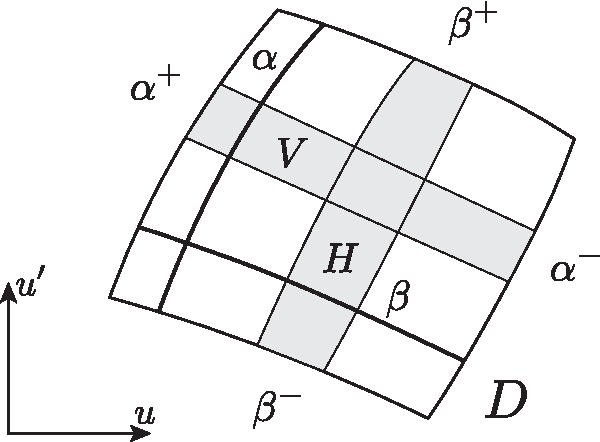
\includegraphics[scale = 1]{pic/curves and strips}
	\caption{An islands $D$ bounded by curves $\alpha^{\pm}$, $\beta^{\pm}$; h-curve $\alpha$, v-curve $\beta$, and two strips: h-strip $H$ and v-strip $V$.}
\label{fig:curves-and-strips}
\end{figure}

All above introduced definitions are illustrated on the figures \ref{fig:islands-set} and \ref{fig:curves-and-strips}.
At last let's define one additional property of island set along with $\mathcal{P}$, $\mathcal{P}^{-1}$ maps.

\begin{definition}
	Let $\mathcal{D}$ be an island set formed by the domains of the $\mathcal{P}$ and $\mathcal{P}^{-1}$ maps that act on this set.
	Consider two islands $D_1, D_2 \in \mathcal{D}$.
	We call the island $D_2$ {\bf forward-reachable} from the island $D_1$ if for any \emph{h}-curve $\alpha \in D_1$ with endpoints lying on the opposite boundaries $\beta_1^{\pm}$ of the island $D_1$ the intersection $\mathcal{P}(\alpha) \cap D_2$ is not empty.
	On the other hand we call the island $D_2$ {\bf backward-reachable} from the island $D_1$ if for any \emph{v}-curve $\beta \in D_1$ with endpoints lying on the opposite boundaries $\alpha_1^{\pm}$ of the island $D_1$ the intersection $\mathcal{P}^{-1}(\beta) \cap D_2$ is not empty.
	Finally we call the island $D_2$ {\bf reachable} from the $D_1$ if it satisfies both forward and backward reachability.
\end{definition}

\begin{remark}
	If an island $D_2$ is forward-reachable from $D_1$ then $D_1$ is backward-reachable from $D_2$ and vice versa.
\end{remark}

\begin{definition}
	We call an island set $\mathcal{D} = \bigcup_{i \in S} D_i$ {\bf complete} if for any $i, j$ island $D_i$ is reachable from $D_j$.
\end{definition}

\subsection{Thickness of strips}

Next we'll also need a definition of the strips thickness.
Let an h-strip $H$ lies inside an island $D$ and is bounded by h-curves $\alpha^+$ and $\alpha^-$.
Consider graphs of that curves as a functions of $u$: $u' = h_{\pm}(u)$.
By the definition $h_{\pm}(u)$ are $\gamma$-Lipschitz function.
Denote by $\Delta^{\pm}$ their domains.
Obviously due to the geometric properties of an island domains $\Delta^{\pm}$ do not coincide except the case when the opposite boundaries $\beta^{\pm}$ lying on the corresponding boundaries of the island $D$ are vertical straight lines.
Let $\Delta^+ = [u_0^+; u_1^+]$, $\Delta^- = [u_0^-; u_1^-]$, consider new domain $\Delta = \Delta^+ \cap \Delta^-$ and define functions $\widetilde{h}_{\pm}(u)$ on the new domain $\Delta$ as follows:
\begin{equation}
	\widetilde{h}_{\pm}(u) = \begin{cases}
		h_{\pm}(u_0^{\pm}) & u < u_0^{\pm}; \\
		h_{\pm}(u) & u \in \Delta^{\pm}; \\
		h_{\pm}(u_1^{\pm}) & u > u_1^{\pm}.
	\end{cases}
\label{eq:continuation}
\end{equation}
Since $h_{\pm}$ are $\gamma$-Lipschitz functions the new functions $\widetilde{h}_{\pm}$ are also $\gamma$-Lipschitz on the whole domain $\Delta$.
Denote by $\widetilde{\alpha}^{\pm}$ the resulted curves formed by the graphs $\widetilde{h}_{\pm}(u)$.

\begin{definition}
	By the {\bf thickness} of an h-strip $H$, denoted $d_h(H)$, we mean the distance between curves $\widetilde{\alpha}^{\pm}$ in C-norm, i.e.
	\begin{equation}
		d_h(H) = d(\widetilde{\alpha}^+, \widetilde{\alpha}^-) = \max \limits_{u \in \Delta} |\widetilde{h}_+(u) - \widetilde{h}_-(u)|.
	\label{eq:h-thickness}
	\end{equation}
\end{definition}

\begin{remark}
	For two \emph{h}-strips $H_1$, $H_2$ the following statement is valid: $H_2 \subseteq H_1 \Rightarrow \Delta_2 \subseteq \Delta_1$ and $d_h(H_2) \le d_h(H_1)$.
\end{remark}

\begin{definition}
	Let maximum of the expression \eqref{eq:h-thickness} is reached at a point $u_*$, i.e.
	\begin{equation}
		u_* = \argmax \limits_{u \in \Delta} |\widetilde{h}_+(u) - \widetilde{h}_-(u)|.
	\label{eq:argmax}
	\end{equation}
	We call an \emph{h}-strip $H$ {\bf well-measurable} if $u_* \in \Delta^+ \cap \Delta^-$.
\label{def:well-measurable}
\end{definition}

\begin{figure}[h]
\centering
	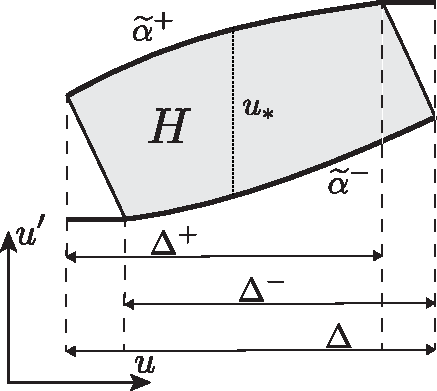
\includegraphics[scale = 1]{pic/thickness definition}
	\caption{An illustration to the definition of an h-strip thickness. Strip $H$ is {\it well-measurable} in a sense of the definition \ref{def:well-measurable}. Curves $\widetilde{\alpha}^{\pm}$ are continuations of the initial h-strip borders to the whole $\Delta$; $u_*$ is a point of maximum of the expression \eqref{eq:h-thickness}.}
\label{fig:thickness-definition}
\end{figure}

\begin{proposition}
	For the \emph{h}-strip $H$ the following statement is valid:
	\begin{equation}
		\Delta^+ \cap \Delta^- \neq \varnothing \Rightarrow u_* \in \Delta^+ \cap \Delta^-,
	\end{equation}
	i.e. an \emph{h}-strip is well-measurable if domains of its border functions have at least one common point.
\end{proposition}
\begin{proof}
	Trivially follows from the monotonicity of the h-strip borders $\alpha^+$ and $\alpha^-$.
\end{proof}

In a similar way we define thickness of v-strips.
Let an v-strip $V$ lies inside an island $D$ and is bounded by v-curves $\beta^+$ and $\beta^-$.
Consider this curves as a functions of $u'$: $u = v_{\pm}(u')$.
Denote domains of these function by $\Delta^{\pm}$.
Continue function $v_{\pm}(u')$ to the whole interval $\Delta = \Delta^+ \cap \Delta^-$ in the same way as for h-strips, see \eqref{eq:continuation}, and introduce new functions $\widetilde{v}_{\pm}(u')$ and curves $\widetilde{\beta}^{\pm}$.

\begin{definition}
	By the {\bf thickness} of an v-strip $V$, denoted $d_v(V)$, we mean the distance between curves $\widetilde{\beta}^{\pm}$ in C-norm, i.e.
	\begin{equation}
		d_v(V) = d(\widetilde{\beta}^+, \widetilde{\beta}^-) = \max \limits_{u' \in \Delta} |\widetilde{v}_+(u') - \widetilde{v}_-(u')|.
	\label{eq:v-thickness}
	\end{equation}
\end{definition}

The definition of {\it well-measurable} v-strip is introduced in a similar manner.
The remark and the proposition above remain valid for the v-strips as well.
Note that thickness of h-strip is measured in a vertical direction, and thickness of v-strip is measured in a horizontal direction.
If a strip is well-measurable then its thickness is measured in a direction along the straight line that connects points from the opposite side of the strip.
This concept will be useful for us during the proof of a theorem about h,v-strips mapping that we'll formulate somewhat below.



\section{Summary}